\documentclass[a4paper,12pt]{report}
\usepackage{graphicx}
\graphicspath{{picaa/}}
\usepackage{listings}
\usepackage{amsmath}
\usepackage[T2A]{fontenc}
\usepackage[utf8]{inputenc}
\usepackage[english,russian]{babel}
\usepackage{pgfplots} 

\usepackage{geometry}
\geometry{left=2cm}
\geometry{right=1.5cm}
\geometry{top=1cm}
\geometry{bottom=2cm}
\lstset{language = Python,
	keywordstyle = \color{orange},
	stringstyle = \color{green},
	commentstyle = \color{red},
	columns = fullflexible
}

\begin{document}

    \begin{titlepage}

        \begin{center}
            \large
            \textbf{Государственное образовательное учреждение высшего профессионального образования\\
            “Московский государственный технический университет имени Н.Э.Баумана”\\}
            
\includegraphics{bmstu-logo.png}
			\vspace{1cm}
            
            \textsc{Дисциплина: Анализ алгоритмов}
            \vspace{0.5cm}
                
            \textsc{Лабораторная работа №3}
            \vspace{1cm}
            
            {\LARGE \textbf{Исследование сложности сортировок}}
            \vspace{3cm}
                    
            \begin{flushright}
            	Студент группы ИУ7-55Б,\\   
            	Руднев К. К.,\\
            	\vspace{0.5cm}
            	Преподаватель,\\
            	Волкова Л. Л.,\\
            	Строганов Ю. В.
            	
            \end{flushright}
            \vfill
            
            2019 г.
            
            \end{center}

    \end{titlepage}

	\setcounter{page}{2}
	\tableofcontents
    \chapter*{Введение}

        	На текущий момент существует огромное количество разнообразных сортировок.
        	Эти алгоритмы необходимо уметь сравнивать, чтобы выбирать наиболее походящий в конкретном случае.\\
        	Эти алгоритмы сравниваются по:
        	\begin{itemize}
        		\item времени сортировки;
        		\item затратам памяти.
        	\end{itemize}
        
			Цель работы: изучение применений алгоритмов сортировки, обучение расчету трудоёмкости алгоритмов.

        \label{sec:intro}

    \newpage

    \chapter{Аналитическая часть}
        \label{sec:analitic_part}

			В рамках раздела будет дано описание гномьей, коктейльной и сортировки выбором.

	\section{Описание алгоритмов}
        
			Сортировка массива - одна из самых популярных операций, проводимых над массивом.
			Алгоритмы реализуют упоядочивание элементов в списке.
			В случае, когда элемент списка имеет несколько полей, поле, служащее критерием порядка, называется ключом сортировки.

	\subsection{Коктейльная сортировка}

    		На каждом шаге основного цикла рассматривается массив array[Left]-array[Right], после выполнения двух внутренних циклов минимальный и максимальный элемент в исходном массиве перетекают к краям, минимальный в — array[Left], максимальный — в array[Right] \cite{Virt_cocktail}.
    		
    \subsection{Сортировка выбором}

    		На каждом i-ом шаге алгоритма находим i-ый минимальный элемент и меняем его местами с i-ым элементом в массиве \cite{Knut_choice}. 
    		Таким образом будет получен массив, отсортированный по неубыванию.
    
    \subsection{Гномья сортировка}

   			Алгоритм находит первое место, где два соседних элемента стоят в неправильном порядке и меняет их местами \cite{Axo_gnome}. 
   			Он пользуется тем фактом, что обмен может породить новую пару, стоящую в неправильном порядке, только до или после переставленных элементов. 
   			Он не допускает, что элементы после текущей позиции отсортированы, таким образом, нужно только проверить позицию до переставленных элементов.

	\section{Вывод}

   			В этом разделе были рассмотрены описания гномьей, коктейльной и сортировки выбором.

    \newpage

    \chapter{Конструкторская часть}
        \label{sec:construct_part}

        	В рамках раздела будут даны схемы алгоритмов для гномьей (рисунок \ref{ris:gnome}), коктейльной (рисунок \ref{ris:cockteil}) и сортировки выбором (рисунок \ref{ris:choice}).

	\section{Разработка алгоритмов}

        \begin{figure}[h!]
        	\centering
        	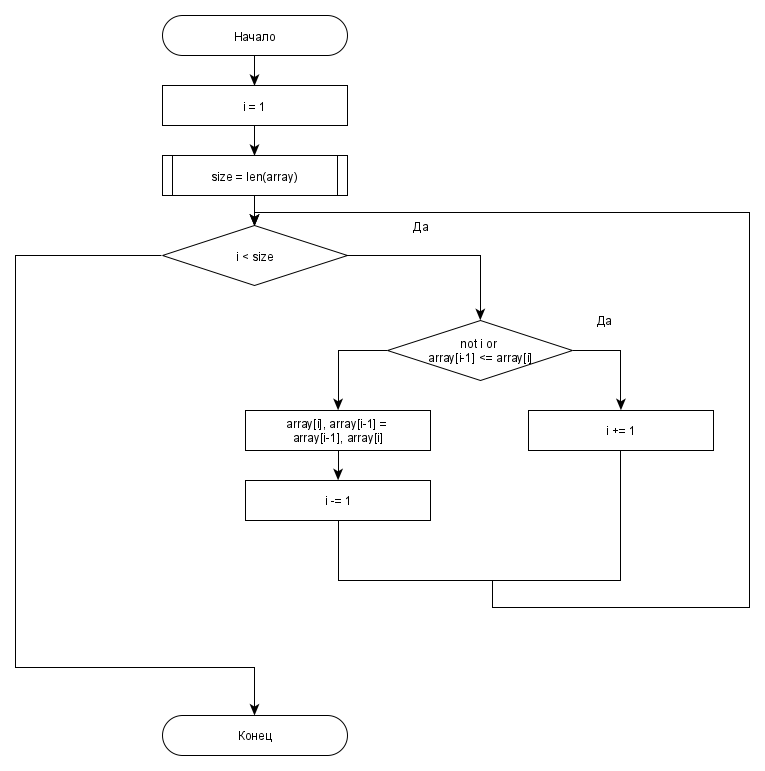
\includegraphics[width=0.8\linewidth]{gnome_sort1.png}
        	\caption{Гномья сортировка}
        	\label{ris:gnome}
        \end{figure}
        
        \newpage
        
        \begin{figure}[h!]
        	\centering
        	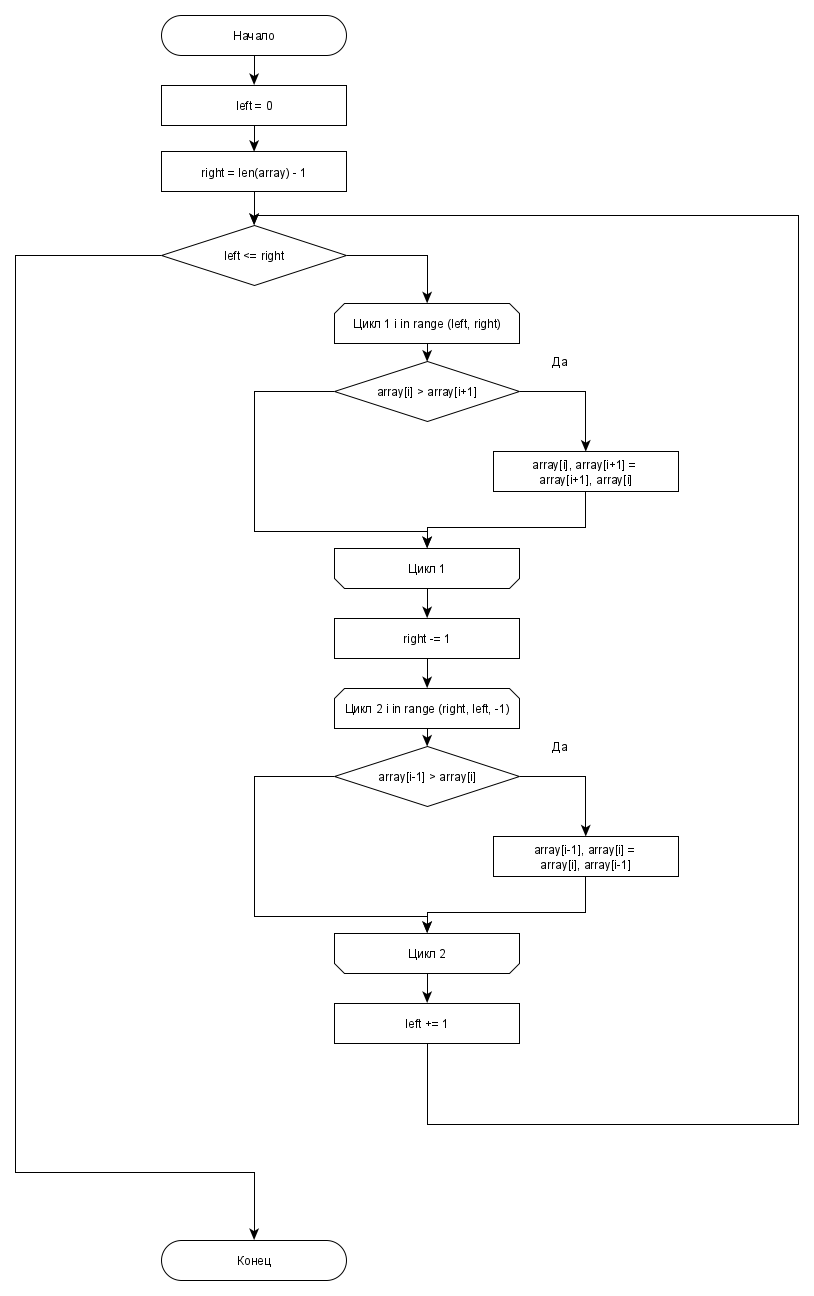
\includegraphics[width=0.8\linewidth]{cocktail_sort1.png}
        	\caption{Коктейльная сортировка}
        	\label{ris:cockteil}
        \end{figure}
    
    	\newpage
    
    	\begin{figure}[h!]
    		\centering
    		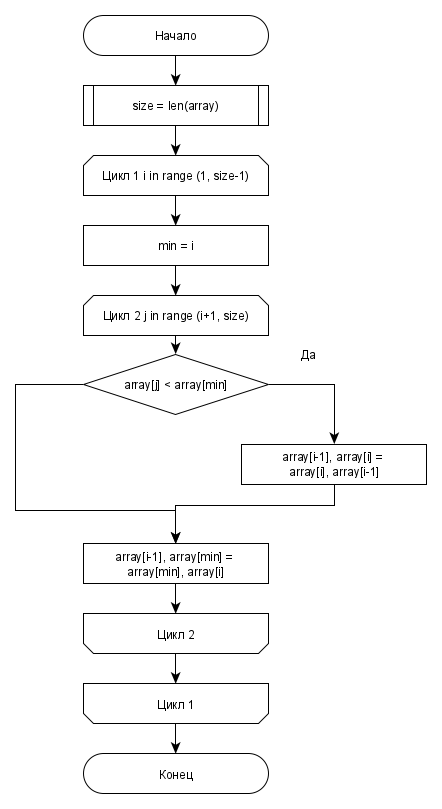
\includegraphics[width=0.65\linewidth]{choice_sort1.png}
    		\caption{Сортировка выбором}
    		\label{ris:choice}
    	\end{figure}
    
    \section{Вывод}
   
    		В этом разделе были рассмотрены схемы алгоритмов коктейльной, гномьей и сортировки выбором.

    \newpage

    \chapter{Технологическая часть}
        \label{sec:tecnologic_part}

        	В рамках раздела будут описаны инструментарии разработки, выбор среды, требования к ПО. 
        	Также будут представлены листинги конкретных реализаций алгоритмов сортировок на рисунках \ref{list:cockteil}-\ref{list:choice}.
        	
        	Замеры времени были произведены на: Intel(R) Core(TM) i7-8565U, 4 ядра, 8 логических процессоров.

	\section{Средства реализации}

        	Для реализации алгоритмов использовался язык программирования Python 3.8.0 и среда разработки PyCharm Community Edition 2019.3.1 by JetBrains. 
        	У меня есть определенный опыт работы с данным языком, которого будет достаточно для реализации текущей лабораторной работы, а среда разработки имеет бесплатную комьюнити версию и удобный интерфейс, упрощающий разработку приложения/скрипта.
        	
        	Замер времени реализован с помощью функции process\_time() библиотеки time.
        	Измеряется время исполнения кода чистого алгоритма (без учета времени на генерацию данных и т.п.).\\
		
	\section{Требования к программному обеспечению}

			На вход программа должна получать массив данных, который сортируется тремя алгоритмами (гномья сортировка, коктейльная сортировка, а также сортировка выбором). 
			
			На выход программа должна выдавать отсортированный по неубыванию массив данных всеми тремя алгоритмами.
			
	\section{Листинг кода}

        	На листинге \ref{list:cockteil} представлена реализация коктейльной сортировки.
        	На листинге \ref{list:gnome} представлена реализация гномьей сортировки.
        	На листинге \ref{list:choice} представлена реализация сортировки выбором.
        	
	        \begin{lstlisting}[frame = single, breaklines, caption = Коктейльная сортировка, label=list:cockteil]
		def cocktail(array):
			left = 0
			right = len(array)-1
			
			while left <= right:
				for i in range(left, right):
					if array[i] > array[i+1]:
						array[i], array[i+1] = array[i+1], array[i]
				right = right - 1
			
				for i in range(right, left, -1):
					if array[i-1] > array[i]:
						array[i-1], array[i] = array[i], array[i-1]
				left = left + 1
			
			return array
	        \end{lstlisting}
	        
	        \begin{lstlisting}[frame = single, breaklines, caption = Гномья сортировка, label=list:gnome]
	       	def gnome(array):
	       		i = 1
	       		size = len(array)
	        	
	       		while i < size:
	        		if not i or array[i - 1] <= array[i]:
	        			i += 1
	        		else:
	        			array[i], array[i - 1] = array[i - 1], array[i]
	        			i -= 1
	        	
	        	return array
	        \end{lstlisting}
	        
	        \begin{lstlisting}[frame = single, breaklines, caption = Сортировка выбором, label=list:choice]
	        def choice(array):
	        	size = len(array)
	        	
	        	for i in range (size - 1):
	        		min = i
	        	
	        		for j in range (i + 1, size):
	        			if array[j] < array[min]:
	        				min = j
	        	
	        		array[i], array[min] = array[min], array[i]
	        	
	        	return array
	        \end{lstlisting}
	        
	\section{Вывод}	
	
		В рамках раздела были предъявлены требования к программному обеспечению. 
		На основании их были разработаны и представлены конкретные реализации всех трёх алгоритмов сортировок.

    \newpage

    \chapter{Экспериментальная часть}
        \label{sec:experimental_part}

			В рамках раздела будут проведены тесты работы программы, представленные на рисунках \ref{ris:test1}-\ref{ris:test3}. 
			Также будут проведены эксперименты, результаты которых представлены на рисунках 4.4-4.6%\ref{graph:sort}-\ref{graph:random}.

	\section{Примеры работы}

        \begin{figure}[h!]
        	\centering
        	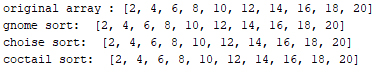
\includegraphics[width=0.9\linewidth]{test_sorted.jpg}
        	\caption{Тест работы сортировок на сортированных массивах}
        	\label{ris:test1}
        \end{figure}
        
        \begin{figure}[h!]
        	\centering
        	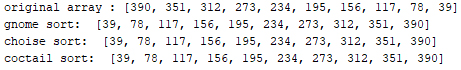
\includegraphics[width=0.9\linewidth]{test_reverse.jpg}
        	\caption{Тест работы сортировок на обратно сортированных массивах}
        	\label{ris:test2}
        \end{figure}
    
    	\begin{figure}[h!]
    		\centering
    		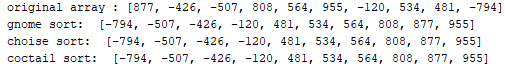
\includegraphics[width=0.9\linewidth]{test_random.jpg}
    		\caption{Тест работы сортировок на случайных массивах}
    		\label{ris:test3}
    	\end{figure}
    
        \newpage
        
    \section{Сравнительный анализ на основе экспериментальных данных}
        
        \begin{figure}[h!]
        \label{graph:sort}
        \begin{tikzpicture}
        \begin{axis}
        [
        	legend pos = north west,
        	ylabel = Время (сек.), xlabel = Размер (элем.),
        	width = 500, height = 400
        ]
        
        \addplot[color=blue] table[x index=0, y index= 1] 
        {cocktail_ord.txt};
        \addlegendentry{Коктейльная сортировка}
        
        \addplot[color=red] table[x index=0, y index= 1] 
        {gnome_ord.txt};
        \addlegendentry{Гномья сортировка}
        
        \addplot[color=green] table[x index=0, y index= 1] 
        {choice_ord.txt};
        \addlegendentry{Сортировка выбором}
        \end{axis}
        \end{tikzpicture}
        \caption{Время выполнения сортировки на упорядоченном массиве}
        \end{figure}
        
        Для всех выбранных сортировок случай отсортированного по возрастанию массива (при условии сортировки по возрастанию) является лучшим случаем. В данной ситуации быстрейшей является гномья сортировка с разницей до 900\%.
        \newpage
        
        \begin{figure}[h!]
        \begin{tikzpicture}
        \begin{axis}
        [
        	legend pos = north west,
        	ylabel = Время (сек.), xlabel = Размер (элем.),
        	width = 500, height = 400
        ]
        
        \addplot[color=blue] table[x index=0, y index= 1] 
		{cocktail_rev.txt};
		\addlegendentry{Коктейльная сортировка}

		\addplot[color=red] table[x index=0, y index= 1] 
		{gnome_rev.txt};
		\addlegendentry{Гномья сортировка}

		\addplot[color=green] table[x index=0, y index= 1] 
		{choice_rev.txt};
        \addlegendentry{Сортировка выбором}
        \end{axis}
        \end{tikzpicture}
        \label{graph:reverse}
        \caption{Время выполнения сортировки на обратно упорядоченном массиве}
    	\end{figure}
        
        Для всех выбранных сортировок случай отсортированного по убыванию массива (при условии сортировки по возрастанию) является худшим случаем. В данной ситуации быстрейшей является сортировка выбором с разницей до 780\%.
        \newpage
        
        \begin{figure}[h!]
        \begin{tikzpicture}
        \begin{axis}
        [
        	legend pos = north west,
        	ylabel = Время (сек.), xlabel = Размер (элем.),
        	width = 500, height = 400
        ]
        
        \addplot[color=blue] table[x index=0, y index= 1] 
        {cocktail_ran.txt};
        \addlegendentry{Коктейльная сортировка}
        
        \addplot[color=red] table[x index=0, y index= 1] 
        {gnome_ran.txt};
        \addlegendentry{Гномья сортировка}
        
        \addplot[color=green] table[x index=0, y index= 1] 
        {choice_ran.txt};
        \addlegendentry{Сортировка выбором}
        \end{axis}
        \end{tikzpicture}
        \label{graph:random}
        \caption{Время выполнения сортировке на случайном массиве}
        \end{figure}
    	В случае случайного массива быстрейшей сортировкой является сортировка выбором с разницей до 233\%.
        
    \section{Оценка трудоёмкости}

       		Считаем, что сортируются массивы размером N.
       		
    \subsection{Модель оценки трудоёмкости}

        Введём систему оценки трудоемкости.

        	\begin{enumerate} 
        		\item Объявление переменной/массива без определения имеет трудоёмкость 0\\
        		\item Операторы +,-,*,/,=, а также +=,-=,// имеют трудоёмкость 1\\
        		\item Оператор доступа по индексу [] имеет трудоёмкость 1\\
        		\item Логические операции имеют трудоёмкость 1\\
        		\item Цикл имеет трудоёмкость 2+N*(2+T), где N - кол-во итераций, T - трудоёмкость тела цикла	
        	\end{enumerate}

	\subsection{Гномья сортировка}

        	\textbf{Лучший случай:} отсортированный массив - получаем это: 2+N-1+N*(1+1+1+1+1)+1 = 7*N+2 $\sim$ O(N) \\
        	
        	\textbf{Худший случай:} отсортированный по убыванию массив - получаем это: 2+($N^{2}$-1)*7+($N^{2}$-1)*9 $\sim$ O($N^{2}$)
        
    \subsection{Сортировка выбором}

        	\textbf{Лучший случай:} отсортированный массив - получаем это: сортировка выбором - устойчивая сортировка, значит:
        	N-1 повторений внешнего цикла, N/2 повторений внутреннего цикла. Тогда $\sim$ O($N^{2}$)\\
        	
        	\textbf{Худший случай:} отсортированный по убыванию массив - получаем это: N-1 повторений внешнего цикла, N/2 повторений внутреннего цикла. Тогда (N-1)*(4+N/2*(4)+5) = (N-1)*(4+2*N+5) = 9*N-9+2*$N^{2}$-2*N = 2*$N^{2}$+7*N-9 $\sim$ O($N^{2}$)

	\subsection{Коктейльная сортировка}

        	\textbf{Лучший случай:} отсортированный массив - получаем это: учитывая, что массив отсортирован, имеем один проход по массиву с линейной сложностью $\sim$ O(N) \cite{Virt_cocktail}\\
        	
        	\textbf{Худший случай:} отсортированный по убыванию массив - получаем это: учитывая, что массив отсортирован по убыванию, имеем сложность $\sim$ O($N^{2}$) \cite{Virt_cocktail}

	\section{Вывод}

			Все сортировки в качестве худшего случая показали квадратичную сложность. 
			В лучшем случае самой быстрой с линейной сложностью оказалась гномья сортировка.
			
			В ходе эксперимента выяснилось, что гномья сортировка позволяет добиться выигрыша до 900\% при сортировке уже отсортированного массива.
			
			Сортировка выбором быстрее до 780\% на обратно отсортированном массиве, а также быстрее на случайном массиве с выигрышем до 233\%.

    \newpage

    \chapter*{Заключение}
        \label{sec:conclusion_part}
        
			В ходе лабораторной работы были изучены алгоритмы сортировки массива: гномья, выбором и коктейльная. 
			Выполнено сравнение всех рассматриваемых алгоритмов. 
			Приведены их трудоемкости. 
			
			В ходе экспериментов выяснилось, что из рассмотренных сортировок гномья сортировка самая быстрая из предложенных в лучшем случае и выигрывает во времени до 900\% на тестовых данных размерностью до 1000 элементов в массиве.
			
			Быстрейшей сортировкой в худшем случае и среднем случае оказалась сортировка выбором. Дает выигрыш до 780\% в худшем и до 233\% в среднем на тестовых данных размерностью до 1000 элементов в массиве.
      
    \begin{thebibliography}{}
	    \bibitem{Virt_cocktail}
	    Н. Вирт Алгоритмы и структуры данных. М., Издат-во "Вильямс", 1998г.
	    \bibitem{Knut_choice}
	    Д. Кнут. Искусство программирования для ЭВМ. Т.3. Сортировка и поиск. М., "Мир", 1978 г., переиздание - М.,Изд-во "Вильямс", 2000 г.
	    \bibitem{Axo_gnome}
	    А. Ахо, Дж. Э. Хопкрофт, Д. Ульман Структуры данных и алгоритмы. М., Изд-во "Вильямс", 2000 г.
	\end{thebibliography}
       
\end{document}
